% Options for packages loaded elsewhere
% Options for packages loaded elsewhere
\PassOptionsToPackage{unicode}{hyperref}
\PassOptionsToPackage{hyphens}{url}
\PassOptionsToPackage{dvipsnames,svgnames,x11names}{xcolor}
%
\documentclass[
  letterpaper,
  DIV=11,
  numbers=noendperiod]{scrartcl}
\usepackage{xcolor}
\usepackage{amsmath,amssymb}
\setcounter{secnumdepth}{-\maxdimen} % remove section numbering
\usepackage{iftex}
\ifPDFTeX
  \usepackage[T1]{fontenc}
  \usepackage[utf8]{inputenc}
  \usepackage{textcomp} % provide euro and other symbols
\else % if luatex or xetex
  \usepackage{unicode-math} % this also loads fontspec
  \defaultfontfeatures{Scale=MatchLowercase}
  \defaultfontfeatures[\rmfamily]{Ligatures=TeX,Scale=1}
\fi
\usepackage{lmodern}
\ifPDFTeX\else
  % xetex/luatex font selection
\fi
% Use upquote if available, for straight quotes in verbatim environments
\IfFileExists{upquote.sty}{\usepackage{upquote}}{}
\IfFileExists{microtype.sty}{% use microtype if available
  \usepackage[]{microtype}
  \UseMicrotypeSet[protrusion]{basicmath} % disable protrusion for tt fonts
}{}
\makeatletter
\@ifundefined{KOMAClassName}{% if non-KOMA class
  \IfFileExists{parskip.sty}{%
    \usepackage{parskip}
  }{% else
    \setlength{\parindent}{0pt}
    \setlength{\parskip}{6pt plus 2pt minus 1pt}}
}{% if KOMA class
  \KOMAoptions{parskip=half}}
\makeatother
% Make \paragraph and \subparagraph free-standing
\makeatletter
\ifx\paragraph\undefined\else
  \let\oldparagraph\paragraph
  \renewcommand{\paragraph}{
    \@ifstar
      \xxxParagraphStar
      \xxxParagraphNoStar
  }
  \newcommand{\xxxParagraphStar}[1]{\oldparagraph*{#1}\mbox{}}
  \newcommand{\xxxParagraphNoStar}[1]{\oldparagraph{#1}\mbox{}}
\fi
\ifx\subparagraph\undefined\else
  \let\oldsubparagraph\subparagraph
  \renewcommand{\subparagraph}{
    \@ifstar
      \xxxSubParagraphStar
      \xxxSubParagraphNoStar
  }
  \newcommand{\xxxSubParagraphStar}[1]{\oldsubparagraph*{#1}\mbox{}}
  \newcommand{\xxxSubParagraphNoStar}[1]{\oldsubparagraph{#1}\mbox{}}
\fi
\makeatother


\usepackage{longtable,booktabs,array}
\usepackage{calc} % for calculating minipage widths
% Correct order of tables after \paragraph or \subparagraph
\usepackage{etoolbox}
\makeatletter
\patchcmd\longtable{\par}{\if@noskipsec\mbox{}\fi\par}{}{}
\makeatother
% Allow footnotes in longtable head/foot
\IfFileExists{footnotehyper.sty}{\usepackage{footnotehyper}}{\usepackage{footnote}}
\makesavenoteenv{longtable}
\usepackage{graphicx}
\makeatletter
\newsavebox\pandoc@box
\newcommand*\pandocbounded[1]{% scales image to fit in text height/width
  \sbox\pandoc@box{#1}%
  \Gscale@div\@tempa{\textheight}{\dimexpr\ht\pandoc@box+\dp\pandoc@box\relax}%
  \Gscale@div\@tempb{\linewidth}{\wd\pandoc@box}%
  \ifdim\@tempb\p@<\@tempa\p@\let\@tempa\@tempb\fi% select the smaller of both
  \ifdim\@tempa\p@<\p@\scalebox{\@tempa}{\usebox\pandoc@box}%
  \else\usebox{\pandoc@box}%
  \fi%
}
% Set default figure placement to htbp
\def\fps@figure{htbp}
\makeatother





\setlength{\emergencystretch}{3em} % prevent overfull lines

\providecommand{\tightlist}{%
  \setlength{\itemsep}{0pt}\setlength{\parskip}{0pt}}



 


\usepackage[most]{tcolorbox}

% Define grey box
\newtcolorbox{grey-bg}{colback=gray!10, colframe=gray!80, boxrule=0.5pt, arc=2pt, left=6pt, right=6pt, top=6pt, bottom=6pt}

% Define red box
\newtcolorbox{red-bg}{colback=red!5, colframe=red!80!black, boxrule=0.5pt, arc=2pt, left=6pt, right=6pt, top=6pt, bottom=6pt}
\KOMAoption{captions}{tableheading}
\makeatletter
\@ifpackageloaded{tcolorbox}{}{\usepackage[skins,breakable]{tcolorbox}}
\@ifpackageloaded{fontawesome5}{}{\usepackage{fontawesome5}}
\definecolor{quarto-callout-color}{HTML}{909090}
\definecolor{quarto-callout-note-color}{HTML}{0758E5}
\definecolor{quarto-callout-important-color}{HTML}{CC1914}
\definecolor{quarto-callout-warning-color}{HTML}{EB9113}
\definecolor{quarto-callout-tip-color}{HTML}{00A047}
\definecolor{quarto-callout-caution-color}{HTML}{FC5300}
\definecolor{quarto-callout-color-frame}{HTML}{acacac}
\definecolor{quarto-callout-note-color-frame}{HTML}{4582ec}
\definecolor{quarto-callout-important-color-frame}{HTML}{d9534f}
\definecolor{quarto-callout-warning-color-frame}{HTML}{f0ad4e}
\definecolor{quarto-callout-tip-color-frame}{HTML}{02b875}
\definecolor{quarto-callout-caution-color-frame}{HTML}{fd7e14}
\makeatother
\makeatletter
\@ifpackageloaded{caption}{}{\usepackage{caption}}
\AtBeginDocument{%
\ifdefined\contentsname
  \renewcommand*\contentsname{Table of contents}
\else
  \newcommand\contentsname{Table of contents}
\fi
\ifdefined\listfigurename
  \renewcommand*\listfigurename{List of Figures}
\else
  \newcommand\listfigurename{List of Figures}
\fi
\ifdefined\listtablename
  \renewcommand*\listtablename{List of Tables}
\else
  \newcommand\listtablename{List of Tables}
\fi
\ifdefined\figurename
  \renewcommand*\figurename{Figure}
\else
  \newcommand\figurename{Figure}
\fi
\ifdefined\tablename
  \renewcommand*\tablename{Table}
\else
  \newcommand\tablename{Table}
\fi
}
\@ifpackageloaded{float}{}{\usepackage{float}}
\floatstyle{ruled}
\@ifundefined{c@chapter}{\newfloat{codelisting}{h}{lop}}{\newfloat{codelisting}{h}{lop}[chapter]}
\floatname{codelisting}{Listing}
\newcommand*\listoflistings{\listof{codelisting}{List of Listings}}
\makeatother
\makeatletter
\makeatother
\makeatletter
\@ifpackageloaded{caption}{}{\usepackage{caption}}
\@ifpackageloaded{subcaption}{}{\usepackage{subcaption}}
\makeatother
\usepackage{bookmark}
\IfFileExists{xurl.sty}{\usepackage{xurl}}{} % add URL line breaks if available
\urlstyle{same}
\hypersetup{
  pdftitle={Technical Note on Queueing Systems},
  colorlinks=true,
  linkcolor={blue},
  filecolor={Maroon},
  citecolor={Blue},
  urlcolor={Blue},
  pdfcreator={LaTeX via pandoc}}


\title{Technical Note on Queueing Systems}
\author{}
\date{}
\begin{document}
\maketitle


\subsection{\texorpdfstring{\textbf{Waiting Times due to Random
Variability}}{Waiting Times due to Random Variability}}\label{waiting-times-due-to-random-variability}

This technical note \textbf{complements} the accompanying video
(\emph{Module 3: Flow and Queue Management}) by offering a rigorous yet
accessible foundation in the principles of queuing systems. It explains
how queues arise, how their performance can be quantified, and what
practical levers managers can use to design better queuing experiences.
While the video builds intuition, this note delivers the mathematical
backbone---clear, targeted, and directly applicable to real-world
operational decisions.

\subsection{\texorpdfstring{\textbf{Introduction: From Lines to
Strategic
Levers}}{Introduction: From Lines to Strategic Levers}}\label{introduction-from-lines-to-strategic-levers}

Whether you're managing a luxury hotel, a call center, or an e-commerce
platform, one operational challenge consistently influences customer
satisfaction and profitability: the queue. Queues are where operations
meet customer experience. They determine perceptions of efficiency,
fairness, and value---and can break or boost loyalty.

As future managers and decision-makers, MBA students must learn to go
beyond intuition and back-of-the-envelope guesses. Queue management is
not just about reducing wait times---it's about managing variability,
optimizing resource allocation, and aligning service delivery with
customer expectations. A short line may reflect good planning---or
overstaffing. A long line may signal high demand---or poor design.

\subsubsection{\texorpdfstring{\textbf{The Key Performance indicators of
Queueing
Systems}}{The Key Performance indicators of Queueing Systems}}\label{the-key-performance-indicators-of-queueing-systems}

Before diving into technical models, it is important to understand the
core performance metrics that service managers need to monitor. In any
system with waiting lines, managers want to understand how many
customers or packages are waiting, how long they wait, how many are
being served or processed, and how long the full experience takes from
arrival to departure. These are expressed as:

\begin{enumerate}
\def\labelenumi{\arabic{enumi}.}
\tightlist
\item
  \emph{Average number of customers/packages waiting in line (denoted
  by} \(L_q\)\emph{- Length of queue)}
\item
  \emph{Average time a customer spends waiting before service (denoted
  by} \(W_q\)\emph{- Waiting time in queue)}
\item
  \emph{Average number of customers in facility (denoted by}
  \(L\)\emph{- Length of queue plus in service)}
\item
  \emph{Average total time a customer spends in the system (denoted by}
  \(W\)\emph{- Waiting time in queue plus being served)}
\end{enumerate}

\begin{tcolorbox}[enhanced jigsaw, colbacktitle=quarto-callout-note-color!10!white, leftrule=.75mm, breakable, bottomtitle=1mm, title=\textcolor{quarto-callout-note-color}{\faInfo}\hspace{0.5em}{At the Airport- Barcelona Prat}, opacitybacktitle=0.6, toptitle=1mm, arc=.35mm, colback=white, rightrule=.15mm, left=2mm, colframe=quarto-callout-note-color-frame, titlerule=0mm, toprule=.15mm, bottomrule=.15mm, opacityback=0, coltitle=black]

Imagine you are managing security operations at Barcelona--El Prat
Airport. As the manager, your objective is to closely monitor key
performance indicators (KPIs) related to queue management. Specifically,
you need to track:

• \textbf{Average Queue Length} \(L_q\): How many passengers are waiting
on average in the security line.

• \textbf{Average Waiting Time in Queue} \(W_q\): How long passengers
wait, on average, before they begin the security check. This KPI
directly impacts how early travelers must arrive at the airport. If
waiting times are expected to be longer than usual, passengers must be
informed promptly to ensure everyone reaches their flights on time.

• \textbf{Average Number of Passengers in the System} \(W\): This
includes passengers currently waiting in line and those actively
undergoing security checks. This measure is directly related to the
space needed.

• \textbf{Average Total Time in the System} \(W\): The overall average
duration passengers spend in the security process, including both
waiting and screening times.

\end{tcolorbox}

These KPIs are crucial because they directly influence outcomes relevant
to managers, including customer satisfaction, labor utilization, service
levels, and operational costs. For instance, in restaurants, seating
delays of thirty minutes negatively affect customer reviews compared to
immediate seating, subsequently impacting future demand. Similarly, in
healthcare settings, prolonged wait times correlate with lower service
ratings and decreased patient retention. Managers frequently confront
the following operational levers:

\begin{itemize}
\item
  \emph{\textbf{Staffing Levels:} How many staff members must I allocate
  to keep the average waiting time within acceptable limits?}
\item
  \emph{\textbf{Queue Design:} Should the queueing system adopt
  dedicated checkouts (like supermarkets), or a single serpentine
  queue?}
\item
  \emph{\textbf{Service Specialization:} Should servers be centralized
  with cross-training, or specialized in specific tasks, and what
  implications will these choices have on key KPIs?}
\end{itemize}

To rigorously provide good estimates of the KPIs and the managerial
levers, we need to understand what influences them.

\subsection{\texorpdfstring{\textbf{Anatomy of a Queueing
system}}{Anatomy of a Queueing system}}\label{anatomy-of-a-queueing-system}

Three elements define any queueing system.

\paragraph{\texorpdfstring{\textbf{Characteristics of Queueing Design
System.}}{Characteristics of Queueing Design System.}}\label{characteristics-of-queueing-design-system.}

The \textbf{structure of the system}, which includes the number of
servers, whether lines are pooled or separate, and how customers are
selected for service. Most systems follow a first-come, first-served
rule, but others may prioritize based on status or need.

\paragraph{\texorpdfstring{\textbf{Characteristics of
Arrivals.}}{Characteristics of Arrivals.}}\label{characteristics-of-arrivals.}

\textbf{Types of items:} While in the service industry we mainly think
of customers as those that arrive to the system, in manufacturing or
distribution settings the arriving items can be packages or material.
Independent of what we are talking about the ``items'' are characterized
by:

\begin{figure}[H]

{\centering 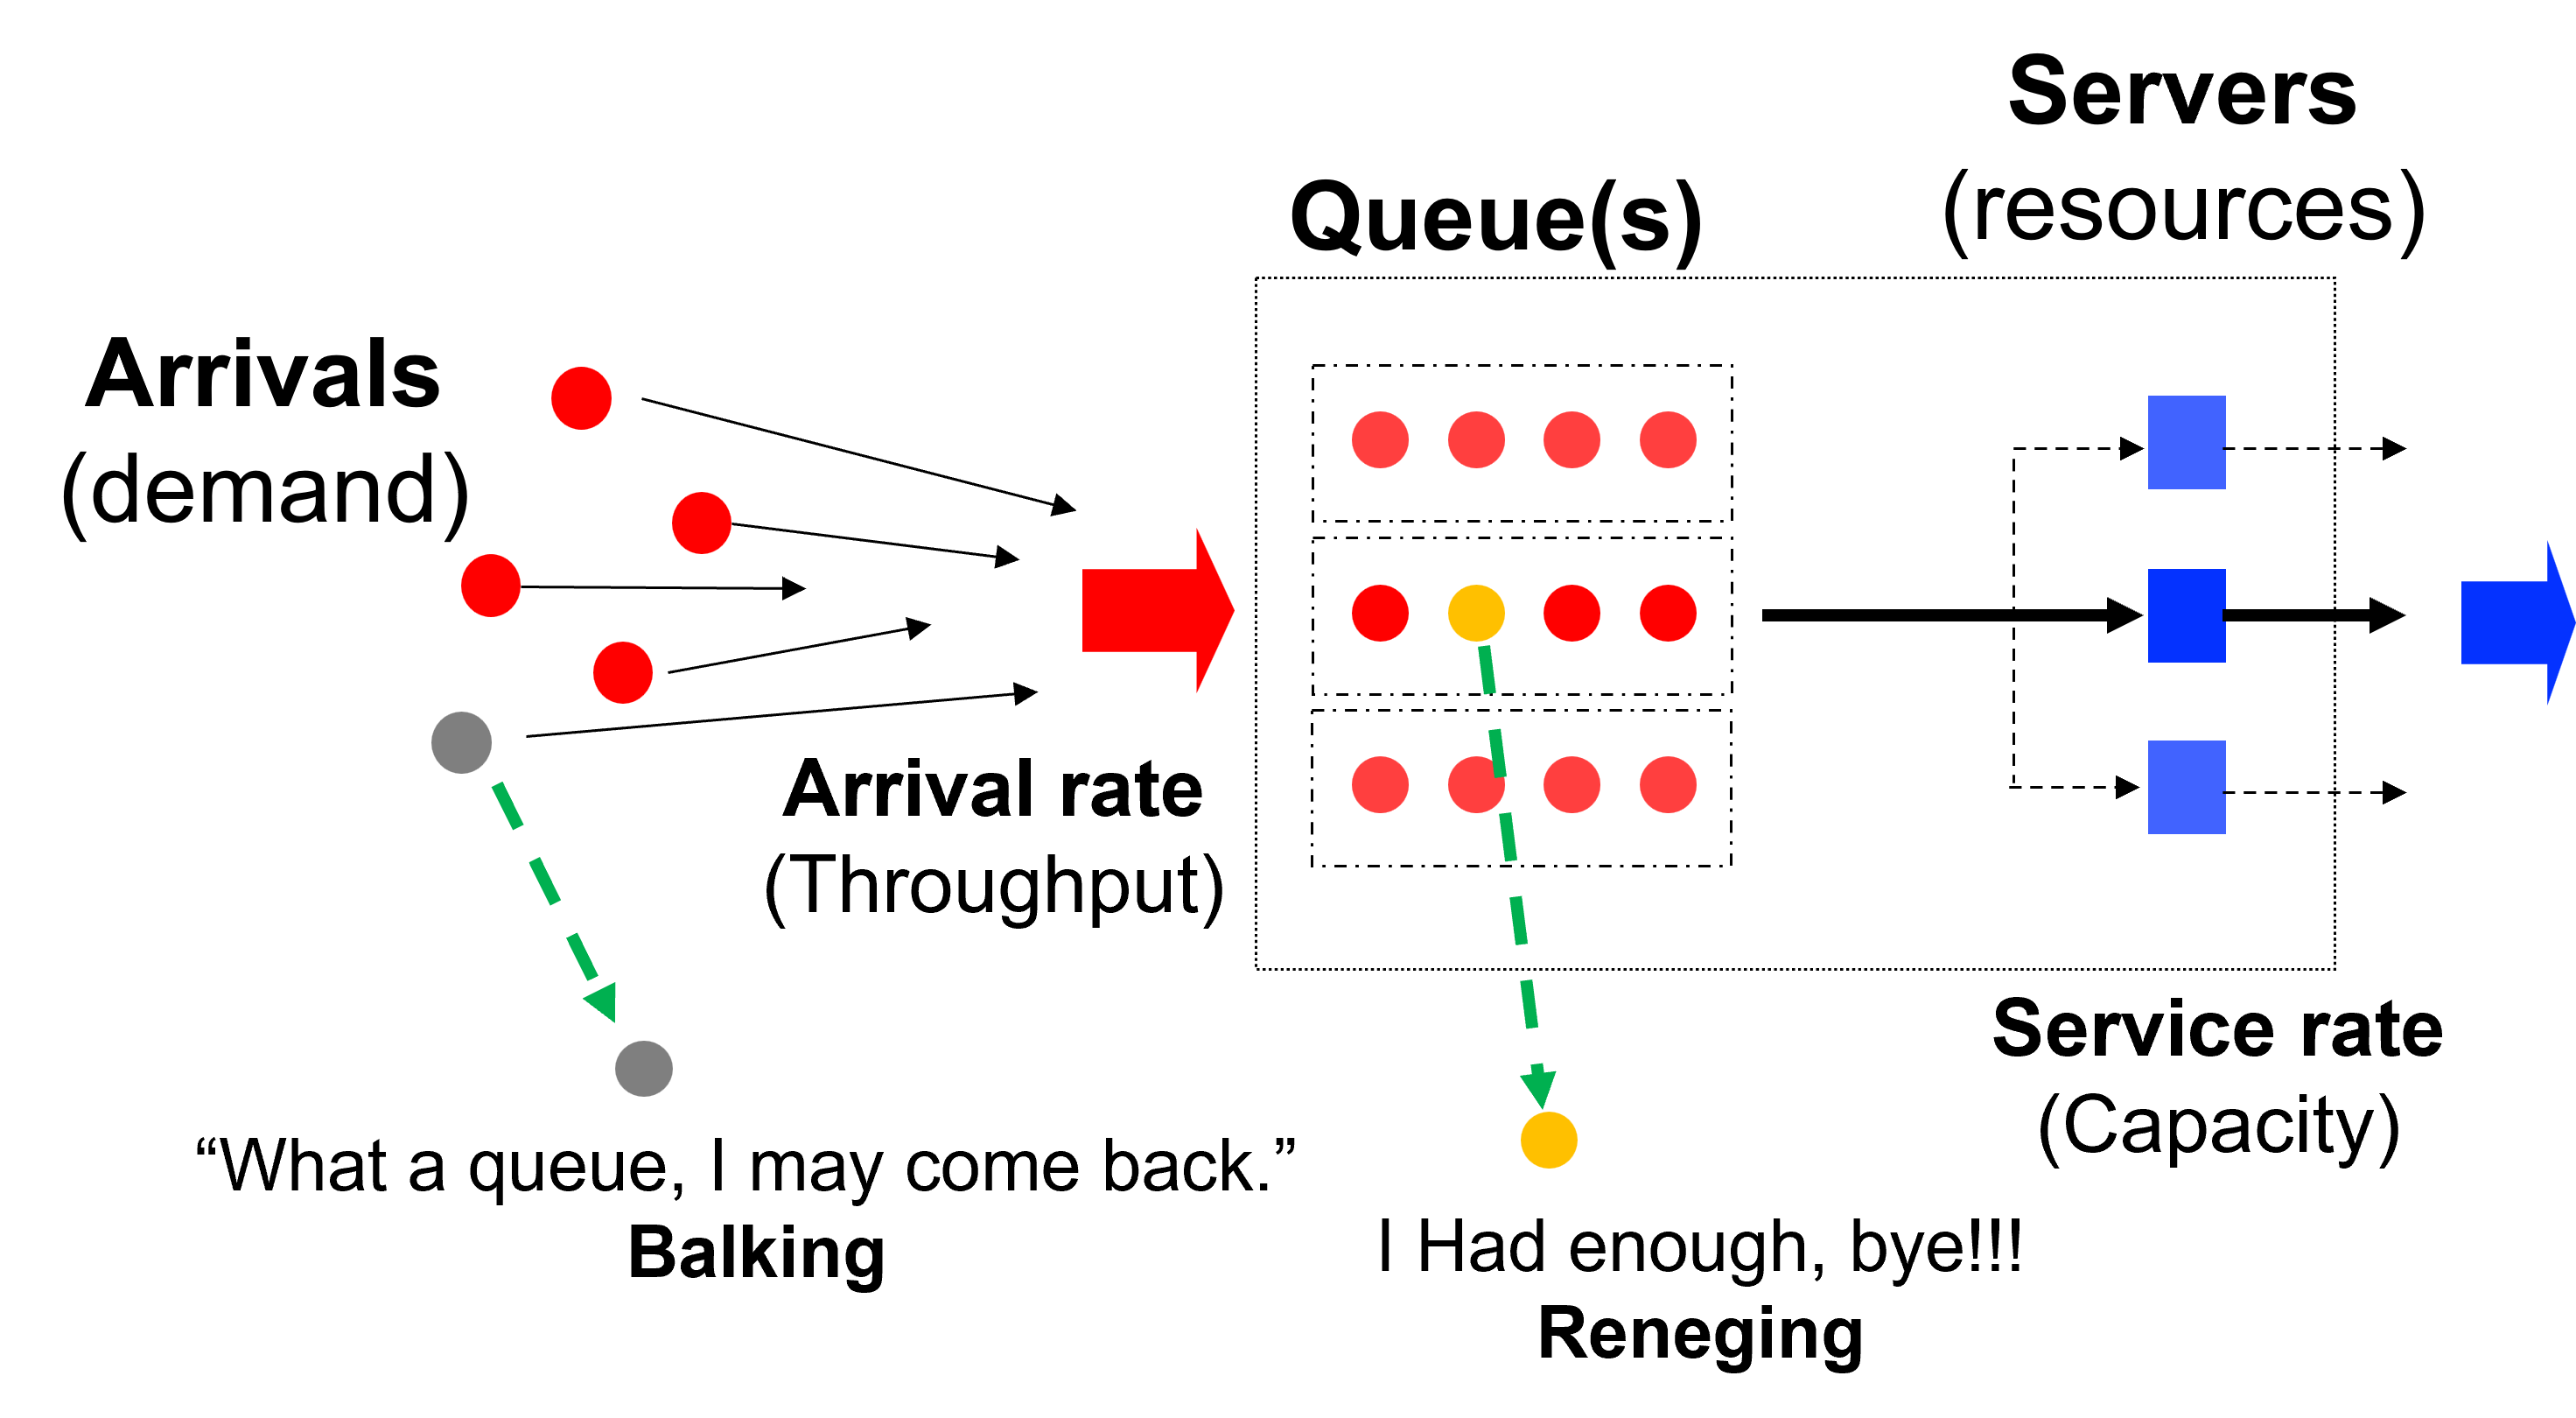
\includegraphics[width=0.5\linewidth,height=\textheight,keepaspectratio]{queueing_representation.png}

}

\caption{Queueing representation}

\end{figure}%

\begin{enumerate}
\def\labelenumi{\alph{enumi})}
\tightlist
\item
  The mean arrival rate (called \(\lambda\) expressed as the number of
  items arriving per unit of time, i.e.~5 customers/hour or by the
  average time between arrivals of \(t_A=12\) min/customer.
\item
  The distribution of arrivals often summarized by the variability or
  standard deviation of interarrival times \(\sigma_A\), i.e.~8 min.
\item
  To understand whether the above mentioned 8 min of standard deviation
  is a lot or not, one standardizes the standard deviation by its mean,
  the so called Coefficient of Variation of arrivals
  \(CV_A=\frac{\sigma}{t_A}=\frac{8}{12}=0.75\). The higher the
  coefficient of variation the more variable a system is.
\end{enumerate}

\paragraph{\texorpdfstring{\textbf{Characteristics of
Servers.}}{Characteristics of Servers.}}\label{characteristics-of-servers.}

\begin{itemize}
\item
  The number of servers an item has available to them once they finished
  waiting in the line. For instance, a typical supermarket where
  customers line up per check out, have typically one server in front of
  them- while a serpentine queueing system where customers could go to
  one of the servers has a multi server system.
\item
  Like arrivals, servers are characterized by the same three service
  time characteristics as the arrivals, namely:

  \begin{itemize}
  \item
    an average service time \(t_S\), i.e 3 min preparation time to make
    a coffee or the capacity of the server \(\mu=\frac{60}{t_s}= 20\)
    coffee per hour.
  \item
    the distribution of service times- or as summary statistics the
    standard deviation \(\sigma_S\) and,
  \item
    the coefficient of variation of service \(CV_S=\sigma_S/t_S\).
  \end{itemize}
\end{itemize}

\begin{tcolorbox}[enhanced jigsaw, colbacktitle=quarto-callout-important-color!10!white, leftrule=.75mm, breakable, bottomtitle=1mm, title=\textcolor{quarto-callout-important-color}{\faExclamation}\hspace{0.5em}{A note on the coefficient of variation (CV)}, opacitybacktitle=0.6, toptitle=1mm, arc=.35mm, colback=white, rightrule=.15mm, left=2mm, colframe=quarto-callout-important-color-frame, titlerule=0mm, toprule=.15mm, bottomrule=.15mm, opacityback=0, coltitle=black]

The coefficient of variation is a unitless measure of relative
variability, defined as the ratio of the standard deviation to the mean
(\(CV_S = \frac{\sigma_S}{t_S}\)). A higher CV (significantly above 1)
indicates high variability (the spread of times is large compared to the
average). A lower CV (closer to 0) indicates low variability and more
predictability. In general,

\begin{itemize}
\item
  \(CV \approx 0\): Deterministic process (no variability).
\item
  \(CV = 1\): Typical of random processes (e.g., customers arriving
  independently).
\item
  \(CV > 1\): Highly variable and unpredictable (chaotic).
\end{itemize}

Managers can use CV to gauge how consistent their arrivals or service
processes are. For example, a very high \(CV_A\) might alert a manager
to highly uneven demand (perhaps suggesting a need for appointments or
reservations), and a high \(CV_S\) might suggest the service process
could be standardized or streamlined to be more consistent, or that the
service in question is very complex and has many different services to
perform.

\end{tcolorbox}

\textbf{Utilization:} In our earlier capacity analysis (without wait
times), we tracked how busy a server or resource was on average. In
queuing analysis, utilization is a key factor: it is the fraction of
time the servers are busy, essentially how much of the system's capacity
is being used by incoming demand. Utilization is defined as:

\[\text{Utilization } (\rho)= \frac{\lambda}{S\times \mu}=\frac{\text{Arrival Rate}}{\text{Number of Servers}\times\text{Service Rate}}\]
This is analogous to the utilization formula in basic capacity analysis.
In words: if you have \(S\) servers each capable of serving \(\mu\)
customers per unit time (so total service capacity is \(S \times \mu\)
per unit time), and customers arrive at rate \(\lambda\), then \(\rho\)
is the fraction of service capacity being utilized by arrivals.

\begin{itemize}
\item
  If \(\rho < 1\), the system can handle the incoming load on average
  (capacity exceeds demand on average). There will be some waiting, but
  the system will eventually catch up with arrivals.
\item
  If \(\rho = 1\), the system is operating at full capacity on average.
  Even a slight random fluctuation can cause the queue to build
  indefinitely (since there's no slack).
\item
  If \(\rho > 1\), the arrival rate exceeds service capacity and the
  queue will explode without bound (the system is fundamentally
  under-capacity).

  Managers should aim to keep \$\textbackslash rho\$ well below 1
  (typically in the 70--90\% range depending on context) to provide a
  buffer for variability and avoid runaway queues.
\end{itemize}

\begin{tcolorbox}[enhanced jigsaw, colbacktitle=quarto-callout-note-color!10!white, leftrule=.75mm, breakable, bottomtitle=1mm, title=\textcolor{quarto-callout-note-color}{\faInfo}\hspace{0.5em}{At the Airport- Barcelona Prat}, opacitybacktitle=0.6, toptitle=1mm, arc=.35mm, colback=white, rightrule=.15mm, left=2mm, colframe=quarto-callout-note-color-frame, titlerule=0mm, toprule=.15mm, bottomrule=.15mm, opacityback=0, coltitle=black]

\textbf{Characteristics of Queueing Design System}:

Let's characterize the security checkpoint system with the parameters
defined:

\textbf{Arrival:}

Suppose roughly \(\lambda= 500\) passengers per hour arrive at the
Terminal 1 security checkpoint during peak times. The standard deviation
of arrivals might be around \(\sigma_A= 500\) passengers/hour (arrivals
fluctuate a lot during the hour), giving
\(CV_A = \frac{500}{500} = 1.0\) (high variability in arrivals).

\textbf{Service:} There are \(S = 10\) security lanes open (servers). On
average, one passenger can be processed in \(t_S = 1\) minute (including
scanning and checks), so each lane has a service rate of \(\mu = 60\)
passengers per hour. The standard deviation of service time might be
around \$\textbackslash sigma\_S = 0.5\$ minutes (30 seconds), so
\$CV\_S = \textbackslash frac\{0.5\}\{1\} = 0.5\$ (service is fairly
consistent, with some variability for different passengers).

\textbf{Arrival.} \emph{Arrival rate:} \(\lambda=500\) passenger/hour

\emph{Standard deviation:} \(\sigma_A=500\) passenger/hour

\emph{Coefficient of Variation}: \(CV_A=500/500=1\)

\textbf{Service}. \emph{Service rate}: \(\mu=1/t_S=60/1\) passenger/hour

\emph{Standard deviation} \(σ_S=0.5\) min/passenger

\emph{Coefficient of Variation:} \(CV_S=0.5/1=0.5\)

\textbf{Utilization}.

Utilization \(\rho=\frac{λ}{S×μ}=\frac{500}{10\times 60}=83\%\). This
means on average \(83\%\) of the security capacity is being used. There
is some spare capacity (17\%), but not a lot -- a surge in arrivals or
slowdown in service could easily create a queue.

\end{tcolorbox}

\textbf{How the KPIs are related (Little's Law)}

Once customers enter a system, how long they stay and how many are
present are not independent. \textbf{Little's Law} provides a simple yet
powerful relationship between throughput, flow time, and inventory in
any steady-state process. Recall from basic operations that we had:

\(WIP=TH\times TT\) (Work in Progress= Throughput rate x Throughput
time)

\begin{figure}[H]

{\centering 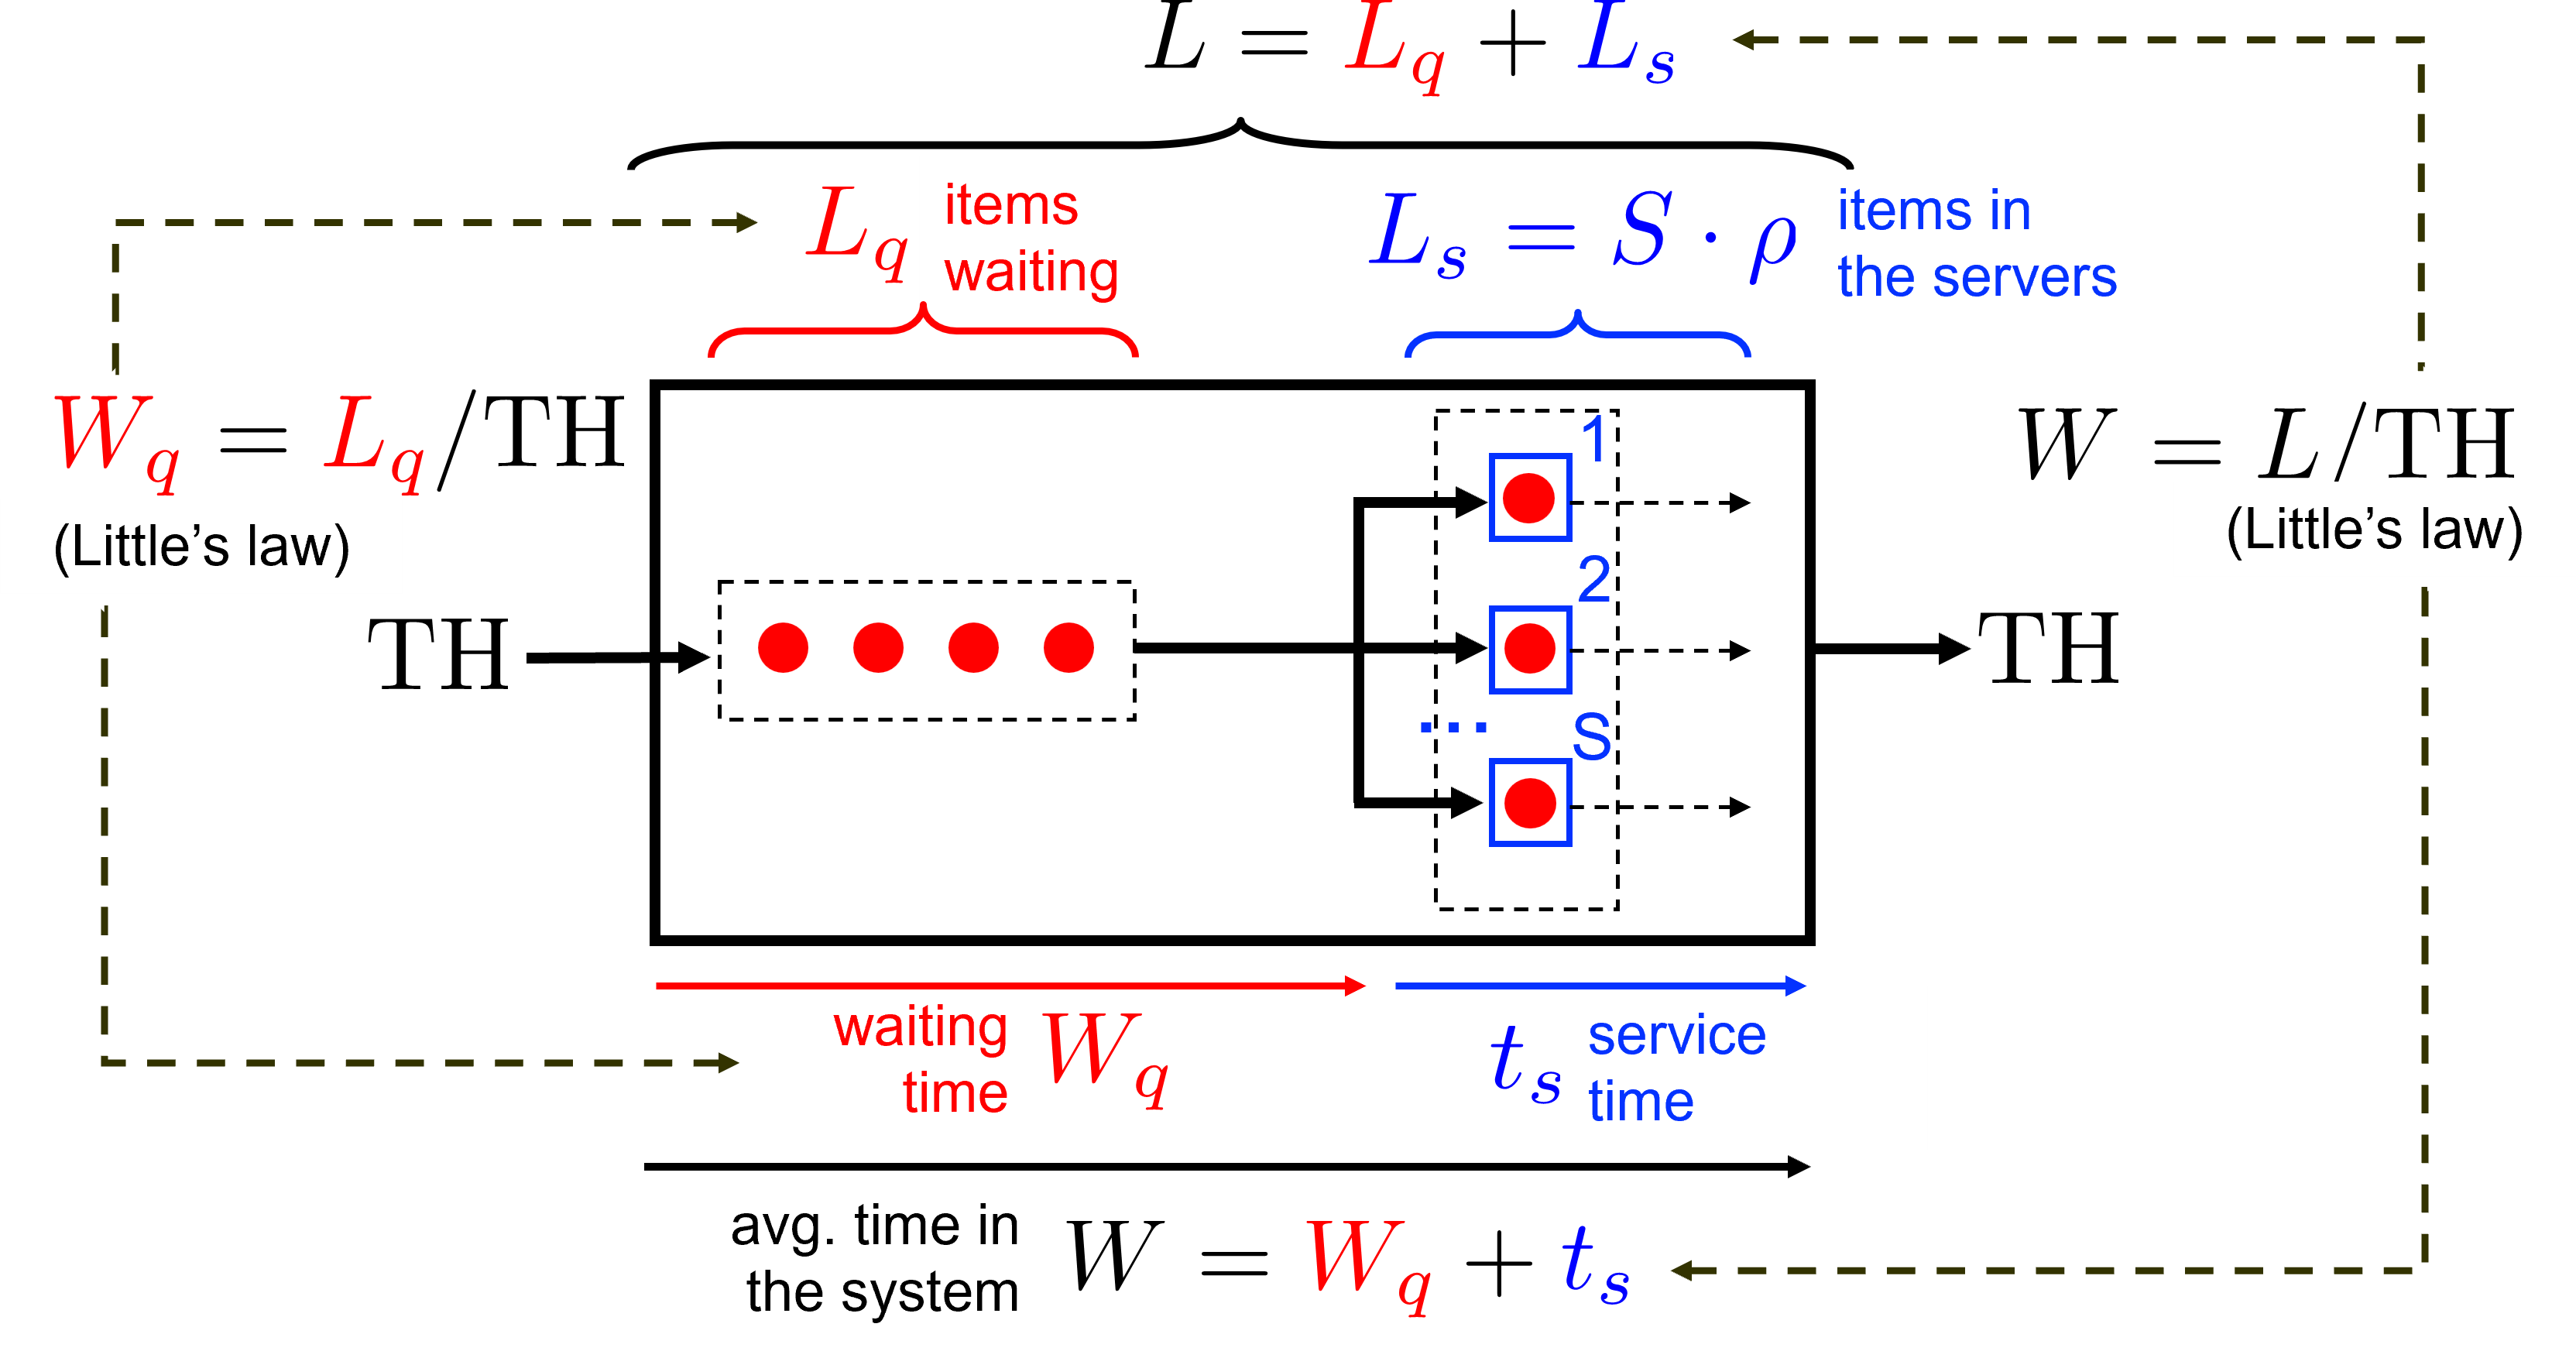
\includegraphics[width=0.5\linewidth,height=\textheight,keepaspectratio]{queueing_KPI.png}

}

\caption{Queueing KPIs}

\end{figure}%

In queueing systems \(WIP\) the number of items that are in the system
is denoted by \(L\) the length of the system, or the number of items in
the system.

The throughput rate, in queueing systems is the arrival rate
(\(\lambda\))- since the arrival rate will be smaller than the service
rate (to ensure that utilization \(\rho<1\)).

The throughput time is the time the item or customer is waiting
\textbf{W.}\\
Thus Little's Law with the queuing terminology can be rewritten as:

\(L=\lambda \times W\) (Length in System= Arrival rate x Total waiting
time)

Or when only considering the queueing system:

\(L_q=\lambda \times W_q\) (Length in Queue= Arrival rate x Waiting time
in queue)

Additionally, and very intuitively we know that the time an item or
customer spends in the system is the time they waited plus the time they
were in service. Mathematically, this can be expressed as:

\(W=w_q+t_S\)

\textbf{Now lets mark what we know from the characterization of a
queueing system:}

\[
L=\textcolor{green}{\lambda} \times W \quad L_q=\textcolor{green}{\lambda} \times W \quad W= W_q + \textcolor{green}{t_S} \quad
\]

Clearly, if we would know one more parameter lets say \(L_q\), then we
could find \(W_q\).

But since we know \(W_q\) we also know \(W\), and if we know \(W\) we
can find \(L\).

Thus in summary, the knowledge of one parameter is sufficient to get all
the KPI's a manager tend to be interested in.

This parameter though must clearly depend on the characteristics of the
queueing system (arrivals, service, and design characteristics). The
formula is an approximation but serves reasonably well to assess
performance of queueing systems.

To estimate \(L_q\) directly, we use the Sakasegawa approximation:

\[
L_q = \frac{\rho^{\sqrt{2 \times (S+1)}}}{1 - \rho} \cdot \frac{CV_A^2 + CV_S^2}{2}
\]

Although not pretty at first and for some even scary, this formula
serves as a fast approximation to estimate queue length, without
restoring to simulation. It's particularly useful in high-level planning
where quick trade-off assessments are needed.

\begin{tcolorbox}[enhanced jigsaw, colbacktitle=quarto-callout-note-color!10!white, leftrule=.75mm, breakable, bottomtitle=1mm, title=\textcolor{quarto-callout-note-color}{\faInfo}\hspace{0.5em}{At the Airport- Barcelona Prat}, opacitybacktitle=0.6, toptitle=1mm, arc=.35mm, colback=white, rightrule=.15mm, left=2mm, colframe=quarto-callout-note-color-frame, titlerule=0mm, toprule=.15mm, bottomrule=.15mm, opacityback=0, coltitle=black]

To calculate the Length of the Queue (\(L_q\)) we need the following:

Utilization \(\rho=83\%\), Number of Servers \(S=10\), Coefficient of
Variation \(CV_A=1, CV_S=0.5\). \[
L_q = \frac{\rho^{\sqrt{2 \times (S+1)}}}{1 - \rho} \cdot \frac{CV_A^2 + CV_S^2}{2}=\frac{0.83^{\sqrt{2\times(10+1)}}}{1-0.83}\frac{1^2+0.5^2}{2}=1.53 \text{ passengers}
\]

With this, we can also calculate the other KPIs:

\textbf{Waiting time in Queue}:
\(W_q=\frac{L_q}{\lambda}=\frac{1.53}{500×3600}=11\) sec.

\textbf{Waiting time in System:} \(W=W_q+t_S=11+60=71\) sec.

\textbf{Number of passengers in System:}
\(L=\lambda \times W= \frac{500}{3600}\times 71= 9.86\) passengers.

\end{tcolorbox}

Now that we've discussed how to derive and interpret key performance
indicators (KPIs) and apply the relevant queueing formula, let's deepen
our understanding by examining its individual components.

The formula for the \textbf{length in the queue} (\(L_q\)) depends on
three crucial characteristics:

\begin{enumerate}
\def\labelenumi{\arabic{enumi}.}
\tightlist
\item
  \textbf{Utilization (}\(\rho\)),
\item
  \textbf{Number of servers (}\(S\)) available for customers,
\item
  \textbf{Coefficient of variation} of arrivals and service times
  (\(CV_A\)), (\(CV_S\)).
\end{enumerate}

We'll now systematically explore how each of these factors independently
influences the length of the queue.

\subsubsection{\texorpdfstring{1. Length in the Queue (\(L_q\)) as a
function of Utilization
(\(\rho\))}{1. Length in the Queue (L\_q) as a function of Utilization (\textbackslash rho)}}\label{length-in-the-queue-l_q-as-a-function-of-utilization-rho}

To simplify our analysis and clearly isolate the effect of utilization,
we temporarily set both the number of servers and coefficients of
variation to 1 (\(S = CV_A = CV_S = 1\)). Our formula for the queue
length reduces neatly to:

\[
L_q = \frac{\rho^{\sqrt{2 \times (S+1)}}}{1 - \rho} \cdot \frac{CV_A^2 + CV_S^2}{2} = \frac{\rho^2}{1 - \rho}.
\]

Below, we illustrate how the queue length \(L_q\) grows as utilization
\(\rho\) increases. We compute \(L_q\) for utilization levels from 0 up
to 0.98 (98\%). Notice that as \(\rho\) approaches 1 (100\%
utilization), the denominator \((1-\rho)\) becomes very small, causing
\(L_q\) to blow up:

\pandocbounded{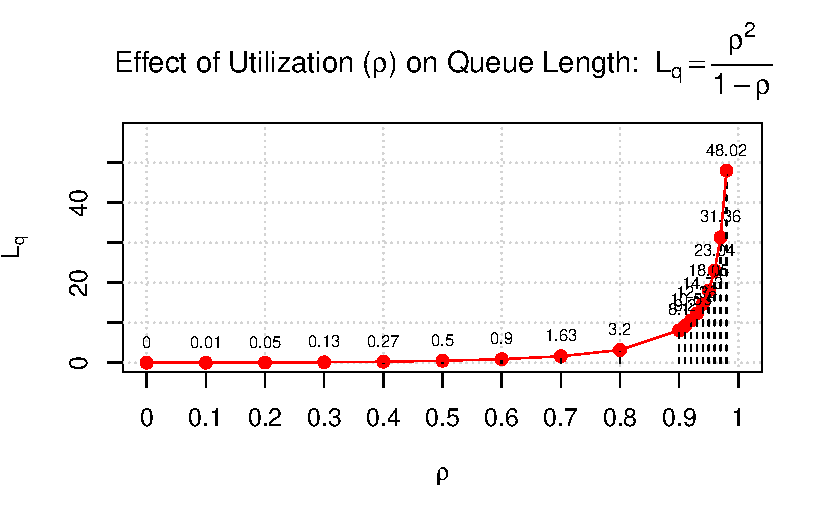
\includegraphics[keepaspectratio]{queueing_technicalnote_files/figure-pdf/one-static-1.pdf}}

As the graph above shows, \textbf{queue length shoots up dramatically as
utilization nears 100\%}. At moderate utilization (say \(\rho = 0.5\) or
\(50\%\) busy), the average queue is quite small. But as you go past

\(80\%\) or \(90\%\), \(L_q\) grows rapidly. For example, increasing
\(\rho\) from \(90\%\) to \(95\%\) might double or triple the queue
length. This has a clear managerial implication: \emph{operating too
close to full capacity is risky}. A system running at more than \(95\%\)
utilization might look efficient on paper (minimal idle time), but it
will likely generate long lines and waiting times that anger customers.
Managers should consider either adding capacity or controlling arrivals
(through appointments, incentives to avoid peak times, etc.) to keep
utilization in a safer range. A rule of thumb is to allow some ``slack''
in the system if customer wait time is a concern.

\subsubsection{\texorpdfstring{2. Length in the Queue (\textbf{\(L_q\)})
as a function of Number of Servers
(S):**}{2. Length in the Queue (L\_q) as a function of Number of Servers (S):**}}\label{length-in-the-queue-l_q-as-a-function-of-number-of-servers-s}

Next, let's examine how the queue length changes as we vary the number
of servers (\(S\)). To clearly illustrate this effect, we'll set the
coefficients of variation (\(CV_A\)) and (\(CV_S\)) both equal to 1, and
explore how (\(L_q\)) behaves as we increase (\(S\)) for a fixed level
of utilization (\(\rho\)).

The simplified formula in this scenario becomes:

\[
L_q = \frac{\rho^{\sqrt{2 \times (S+1)}}}{1 - \rho} \cdot \frac{CV_A^2 + CV_S^2}{2} = \frac{\rho^{\sqrt{2\times(S+1)}}}{1-\rho}
\]

Below, we show how the queue length (\(L_q\)) decreases as we increment
the number of servers (\(S\)) from 1 up to 10, highlighting how
additional servers reduce congestion and improve customer experience.

\pandocbounded{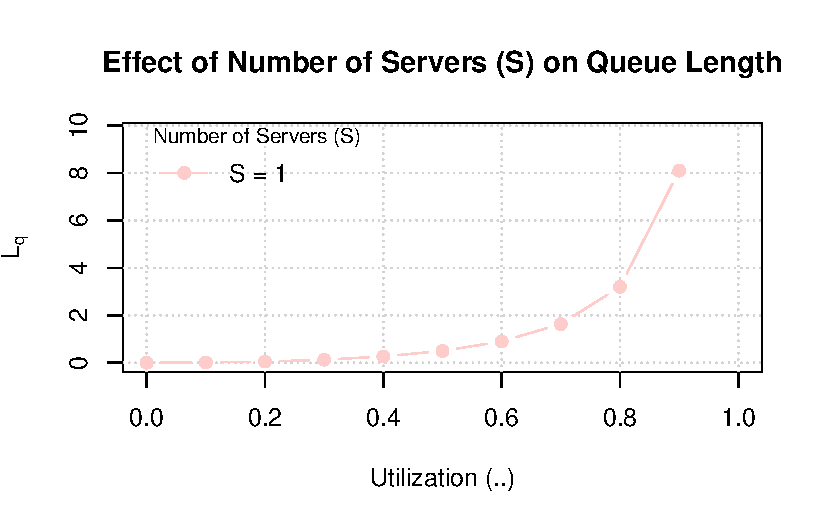
\includegraphics[keepaspectratio]{queueing_technicalnote_files/figure-pdf/second-static-1.pdf}}

\pandocbounded{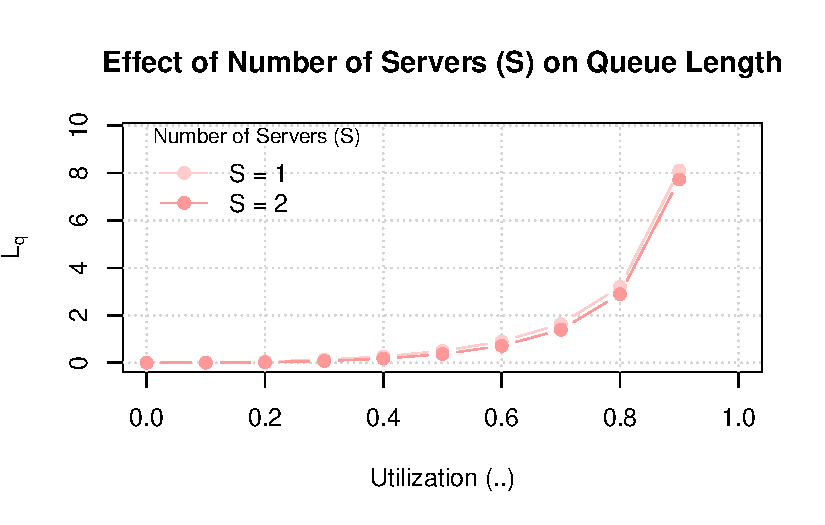
\includegraphics[keepaspectratio]{queueing_technicalnote_files/figure-pdf/second-static-2.pdf}}

\pandocbounded{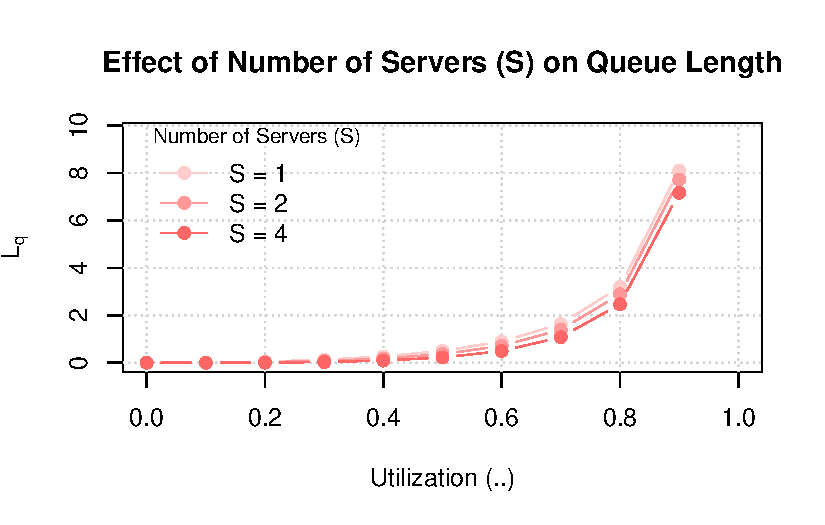
\includegraphics[keepaspectratio]{queueing_technicalnote_files/figure-pdf/second-static-3.pdf}}

\pandocbounded{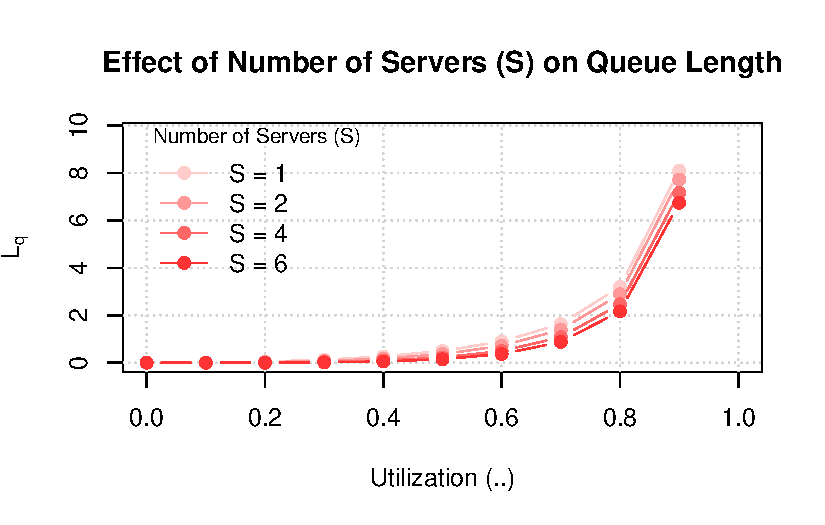
\includegraphics[keepaspectratio]{queueing_technicalnote_files/figure-pdf/second-static-4.pdf}}

\pandocbounded{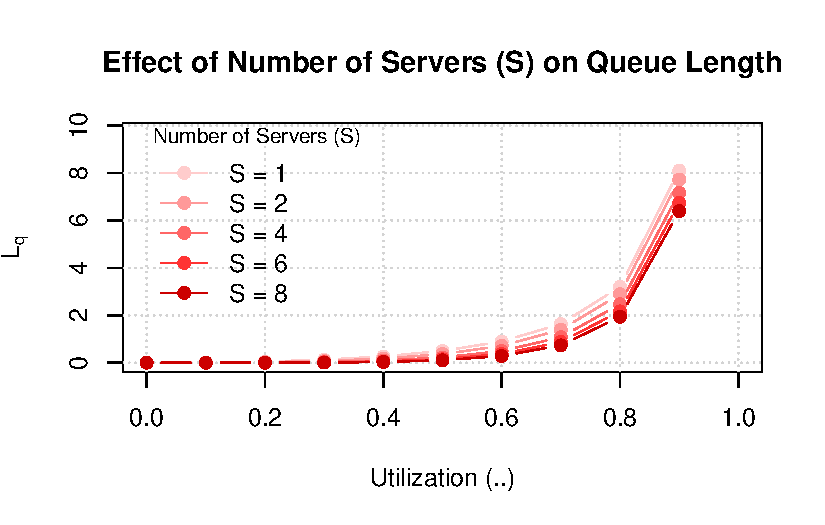
\includegraphics[keepaspectratio]{queueing_technicalnote_files/figure-pdf/second-static-5.pdf}}

\pandocbounded{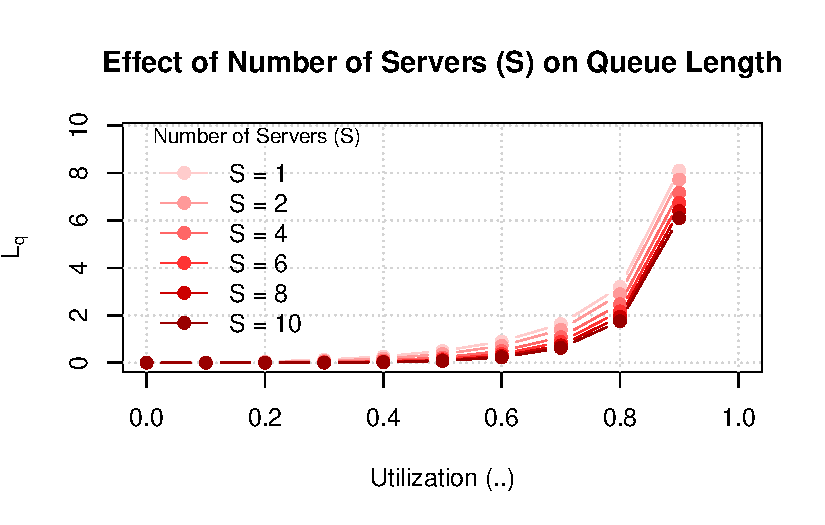
\includegraphics[keepaspectratio]{queueing_technicalnote_files/figure-pdf/second-static-6.pdf}}

\subsubsection{\texorpdfstring{3. Length in the Queue (\textbf{\(L_q\)})
as a function of Coefficient of Variations
(\textbf{\(CV\)}):**}{3. Length in the Queue (L\_q) as a function of Coefficient of Variations (CV):**}}\label{length-in-the-queue-l_q-as-a-function-of-coefficient-of-variations-cv}

Finally, let's examine how the queue length changes as we vary the
coefficient of variations (\(CV\)). To do this let us focus on the
coefficent of variations for arrivals \(CV_A\) and for illustrative
purposes let the coefficient of variations of service be \(CV_S=0\).
Furthermore, as before we let the number of servers be \(S=1\). In this
case the approximation formula simplifies to:

\[
L_q = \frac{\rho^{\sqrt{2 \times (S+1)}}}{1 - \rho} \cdot \frac{CV_A^2 + CV_S^2}{2} = \frac{\rho^{2}}{1-\rho}\cdot\frac{CV_A^2}{2} 
\]

\pandocbounded{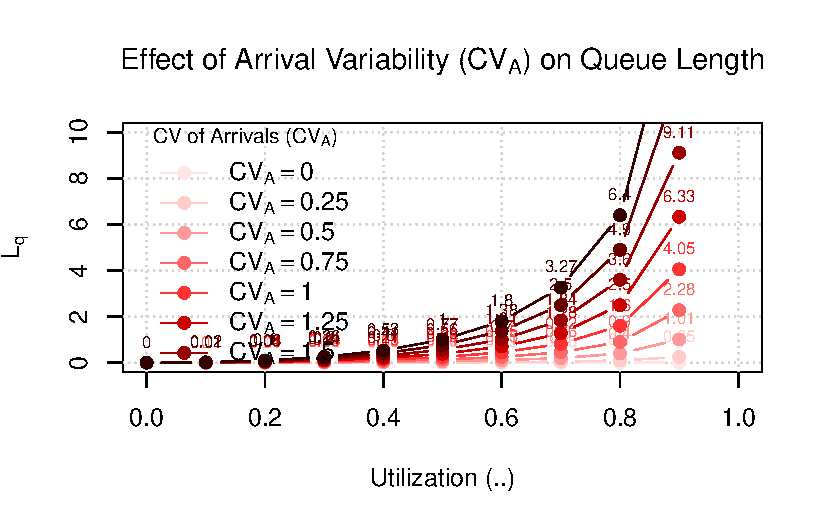
\includegraphics[keepaspectratio]{queueing_technicalnote_files/figure-pdf/third-static-1.pdf}}

The chart illustrates that \textbf{lower variability leads to shorter
queues} for the same average utilization. In the extreme case
(\(CV_A = 0\), the dark red line), arrivals are perfectly steady (e.g.,
exactly one customer every fixed interval). Here, you see that \(L_q\)
remains very low up until extremely high utilizations because the system
is not experiencing any random surges -- customers arrive like clockwork
and are processed in an orderly fashion. On the other hand, the top line
(\(CV_A = 1.0\), light red/pink) shows much higher queues at moderate
utilizations because arrivals can bunch up randomly (for example, you
might get 5 customers arriving almost at once, then a gap, etc., causing
a backlog).

\textbf{Managerial insight:} Reducing variability is a powerful lever
for improving queue performance. While variability is sometimes outside
your direct control (e.g., random customer walk-ins), there are ways to
manage it:

\begin{itemize}
\item
  \emph{Arrival variability:} Can be mitigated by smoothing demand. For
  instance, use appointment systems, require reservations, offer
  incentives for customers to come at off-peak times, or use queue
  management tools that meter entry (e.g., allowing a certain number of
  people into a system per minute).
\item
  \emph{Service time variability:} Can be reduced by standardizing
  procedures, training staff to a consistent performance level, or
  segmenting customers by service requirements (so that simple tasks are
  handled in one line, complex tasks in another, ensuring that a single
  slow transaction doesn't hold up everyone behind them).
\item
  \emph{Buffering variability:} Even if you can't reduce inherent
  variability, you can buffer against it -- for example, having a
  \textbf{pool} of servers/agents that can be activated when there's a
  sudden surge (on-call staff or multi-skilled employees who can jump
  in).
\end{itemize}

Reducing variability has a similar effect to increasing capacity: it
cuts down wait times. In some cases, it might even be more
cost-effective -- e.g., smoothing out an appointment schedule costs
nothing but can eliminate the need to hire an additional full-time staff
member just to handle unpredictable peaks.

\subsection{\texorpdfstring{\textbf{Managerial Levers: Designing a
Better
Queue}}{Managerial Levers: Designing a Better Queue}}\label{managerial-levers-designing-a-better-queue}

In summary, managers have \textbf{three major levers} to improve queue
performance and customer experience:

\begin{enumerate}
\def\labelenumi{\arabic{enumi}.}
\item
  \textbf{Add Capacity (Increase Servers or Service Rate):} If wait
  times are too high, one solution is to increase the service capacity.
  This could mean adding more servers (staff, checkout lanes, call
  center agents, etc.) or improving service rates (training staff to
  work faster, introducing self-service kiosks to handle simpler tasks,
  etc.). The impact of this lever is directly seen in utilization
  \(\rho\): more capacity means lower \(\rho\) for the same arrival
  rate, which prevents the explosive growth of queues as shown earlier.
  \emph{Trade-off:} Additional capacity incurs higher costs (labor,
  equipment). A manager must balance the cost of extra capacity against
  the benefit of shorter queues (and the improved customer satisfaction
  or higher throughput that results).
\item
  \textbf{Reduce Variability (Stabilize Arrivals/Service):} As we saw,
  high variability in demand or service times amplifies queues. Managers
  can implement strategies to smooth demand (reservations, appointments,
  dynamic pricing to shift demand, etc.) and streamline service
  (standard operating procedures, training for consistency, or even
  small process improvements like having paperwork filled in advance).
  Reducing variability (lower \(CV_A\) and \(CV_S\)) makes the system
  more predictable and queue lengths more manageable. \emph{Trade-off:}
  It may require operational changes or enforce restrictions on
  customers (which need to be managed carefully to avoid inconvenience).
  For example, requiring appointments can level demand but might deter
  spontaneous customers.
\item
  \textbf{Pooling and Flexibility:} \textbf{Pooling} means combining
  queues or resources so that variability is shared. Instead of two
  separate queues for two servers (where one server might be idle while
  the other has a line), a single pooled queue ensures both servers are
  almost always busy when there is demand, and customers are served in
  order. Pooling greatly reduces the probability that one server is
  starving while another is overwhelmed. Similarly, cross-training staff
  (flexibility) means employees can shift to where the need is highest,
  effectively creating a pooled resource. Pooling \textbf{reduces the
  impact of variability} because fluctuations even out across a larger
  system. For managers, this could mean using a common queue for all
  checkouts, having a universal call center instead of dedicated lines
  for each region, or deploying ``floaters'' who can assist wherever a
  line starts forming. \emph{Trade-off:} Pooled systems can sometimes
  feel less personal, and cross-training staff requires broader skills
  (and possibly higher wages). Also, customers might perceive a single
  long queue as worse than multiple shorter ones, even if the wait time
  is the same, so communication and expectation management are key.
\end{enumerate}

Finally, it's worth remembering that \textbf{queues are symptoms of
deeper issues} in operations design. A smart manager doesn't just fight
fires by yelling at employees to work faster when lines get long;
instead, they \textbf{redesign the system}. This technical note
introduced key concepts and formulas to \emph{quantitatively} analyze
queues. Using these insights, managers can move from reactive to
proactive management. By anticipating how utilization and variability
interact to create waits, and by leveraging capacity and pooling
strategically, you can design service systems that keep waits within
acceptable limits. The result: \textbf{happier customers, more efficient
operations, and a healthier bottom line}.




\end{document}
